
\documentclass[tikz, border=2pt]{standalone}
\usepackage{tikz}
\begin{document}
    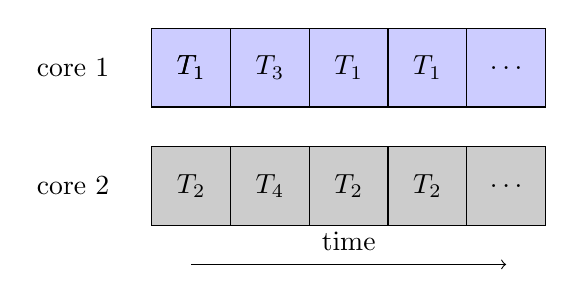
\begin{tikzpicture}
        \foreach \x in {1,...,5}
        {    
            \draw [fill=blue!20] (\x,1.5) rectangle (\x+1,2.5);
            \draw [fill=black!20] (\x,0) rectangle (\x+1,1);
        }
        \draw [->] (1.5,-0.5) -- (5.5,-0.5);
        \node [align=center] at (3.5, -0.2) {time};
        \node [align=center] at (0, 2) {core 1};
        \node [align=center] at (0, 0.5) {core 2};
        \node [align=center] at (1.5, 2) {$T_1$};
        \node [align=center] at (1.5, 0.5) {$T_2$};
        \node [align=center] at (2.5, 2) {$T_3$};
        \node [align=center] at (2.5, 0.5) {$T_4$};                        
        \node [align=center] at (1.5, 2) {$T_1$};
        \node [align=center] at (3.5, 2) {$T_1$};
        \node [align=center] at (3.5, 0.5) {$T_2$};  
        \node [align=center] at (4.5, 2) {$T_1$};
        \node [align=center] at (4.5, 0.5) {$T_2$};
        \node [align=center] at (5.5, 2) {$\dots$};
        \node [align=center] at (5.5, 0.5) {$\dots$};  
    \end{tikzpicture}
\end{document}